\documentclass[12pt,twoside]{article}
\usepackage[dvipsnames]{xcolor}
\usepackage{tikz,graphicx,amsmath,amsfonts,amscd,amssymb,bm,cite,epsfig,epsf,url}
\usepackage[hang,flushmargin]{footmisc}
\usepackage[colorlinks=true,urlcolor=blue,citecolor=blue]{hyperref}
\usepackage{amsthm,multirow,wasysym,appendix}
\usepackage{array,subcaption} 
% \usepackage[small,bf]{caption}
\usepackage{bbm}
\usepackage{pgfplots}
\usetikzlibrary{spy}
\usepgfplotslibrary{external}
\usepgfplotslibrary{fillbetween}
\usetikzlibrary{arrows,automata}
\usepackage{thmtools}
\usepackage{blkarray} 
\usepackage{textcomp}
\usepackage[left=0.8in,right=1.0in,top=1.0in,bottom=1.0in]{geometry}
\newcommand{\ry}{\rnd{ y}  }
\newcommand{\rx}{\rnd{ x}  }
\newcommand{\ru}{\rnd{ u}  }
\newcommand{\rd}{\rnd{ d}  }
%\newcommand{\rs}{\rnd{ s}  }
\newcommand{\ri}{\rnd{ i}  }
\newcommand{\re}{\rnd{ e}  }
\newcommand{\rQ}{\rnd{ q}  }
\newcommand{\rC}{\rnd{ c}  }
\newcommand{\rnd}{\Tilde}
\newcommand{\Id}{Id}
\newcommand{\R}{\mathbb{R}}



\usepackage{pdfpages}
\title{Linear Algebra HW 12}
\author{gjd9961}
\date{December 4th 2021}

\begin{document}
\maketitle
\section{Problem 12.1}The following plot shows the contour lines of a function $f:\R^2 \to \R$.\\
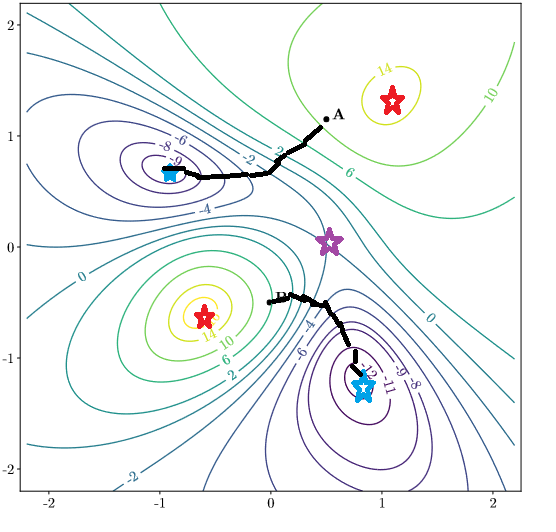
\includegraphics[scale=1]{image.png}

\newpage

a) Give (approximately) the coordinates of the global/local minimizers/maximizers, saddle points of $f$.\\

I marked the local minimums with blue stars, local maxima with red stars. The saddle point is marked with a purple star, and the path that gradient descent would take from either point A or point B is marked with a black line.\\

The coordiantes of the critical points are approximately as follows:
\begin{enumerate}
    \item Global Minimum Approx. $(\frac{4}{5},\frac{-5}{4})$
    \item Local Minimum: Approx. $(\frac{4}{5},\frac{-5}{4})$ and Approx. $(\frac{-7}{8},\frac{2}{3})$
    \item Global Maximum: Approx. $(\frac{-2}{3},\frac{-2}{3})$
    \item Local Maximum: Approx. $(\frac{-2}{3},\frac{-2}{3})$ and Approx. $(\frac{5}{4},\frac{5}{4})$
    \item Saddle Point: Approx. $(\frac{1}{2},0)$
    
\end{enumerate}
b) Assume that we run gradient descent to minimize $f$. Will gradient descent converge to the global minimizer of $f$ when initialized at point $\bbf{A}$ or at point $\bbf{B}$? \\

We can look at the counter plot and begin at either point either A or B. For point A, if we follow the gradient that is orthogonal to the counter lines, we can see that we get trapped in the local minimum at $(\frac{-7}{8},\frac{2}{3})$ and will not reach the global minimum.

Conversely, we can see that if we start at point B, we will follow the orthogonal gradient to the counter lines and approach the global minimum at point $(\frac{-2}{3},\frac{-2}{3})$. 

\vspace{5mm}

\section{Problem}
	Let $M \in \R^{d \times d}$ be a positive semidefinite matrix, $b \in \R^d$ and $c \in \R$. We aim at minimizing the quadratic function
	$$
	f(x) = \frac{1}{2} x^{\sT} M x - \langle x,b \rangle + c
	$$
	using gradient descent. 
	We assume that $M$ is positive definite (i.e.\ all its eigenvalues are positive).
	We let $\lambda_1 \geq \lambda_2 \geq \cdots \geq \lambda_d >0$ be its eigenvalues and let $v_1, \dots, v_d$ be an orthonormal basis of $\R^d$ consisting of associated eigenvectors ($Mv_i = \lambda_i v_i$ for all $i$).
	We write $L = \lambda_1$ and $\mu = \lambda_d$.
	\\

	We consider standard gradient descent with constant step-size $\beta$:
$$
x_{t+1} = x_t - \beta \nabla f(x_t).
$$

a) Show that $f$ is $L$-smooth, $\mu$-strongly convex and that $x^* = M^{-1} b$ is the unique minimizer of $f$.\\

We can take advantage of a few facts given to us in the problem. Firstly, lets calculate the gradient and Hessian of our function $f(x)$:
$$
    \nabla f(x) = f'(x) = Mx - b
$$
The Hessian can be computed as follows:
$$
    H_{f(x)}= M
$$
Setting the gradient equal to 0 we can calculate a minimizer for our function:
\begin{equation}
    \begin{split}
        \nabla f(x) = 0\\
        Mx - b = 0\\
        x = M^{-1}b \qed
    \end{split}
\end{equation}
We know this solution is unique as our Hessian is Positive Definite since its equal to the Positive Definite matrix M. Therefore, there is no null space, and the matrix M is invertible, thus M is a deterministic linear transformation. \\

As for the properties of $f$ being L-smooth and $\mu$-strongly convex, these are both true by definition of the problem statement, as $\mu = \lambda_d$ and $L= \lambda_1$. As we know $\lambda_1 \geq \lambda_2 \geq \cdots \geq \lambda_d >0$, we have shown that the function $f$ satisfies the properties of being L-smooth and $\mu$-strongly convex.\\

b) We now study the convergence of gradient descent to $x^*$. Show that for all $t \geq 0$,
			$$
			x_{t+1} - x^* = \big(\Id - \beta M \big)(x_t - x^*).
			$$
The answer follows from the definition of standard gradient descent defined in the problem statement, and our calculations from part a that showed that the gradient is: $\nabla f(x) = Mx-b$, and therefore $\nabla f(x) + b = Mx$ 
\begin{equation}
    \begin{split}
        x_{t+1} - x^* &= \big(\Id - \beta M \big)(x_t - x^*)  \text{ definition} \\
        x_{t+1} - x^* &= Id_n x_{t} - Id_nx^* - \beta Mx_{t} + \beta Mx^*  \text{ foil function} \\
        x_{t+1} - x^* &= x_{t} - x^* + \beta b - \beta\nabla f(x_t) - \beta b  + \beta\nabla f(x^*)  \text{ gradient plus b equals Mx} \\
        x_{t+1} - x^* &= x_{t} - \beta\nabla f(x_t) - x^* \text{ definition of standard gradient descent} \\
        x_{t+1} - x^* &= x_{t+1} - x^* \qed
    \end{split}
\end{equation}
c)From now, we set $\beta = 1/L$. Deduce from the previous question that for all $t \geq 0$
			$$
			\|x_t - x^* \| \leq \Big(1- \frac{\mu}{L}\Big)^{\! t} \, \|x_0 - x^*\|.
			$$
We can generalize the result of our previous computation to hold for any arbitary $t$. We take the following:
	$$
			x_{t+1} - x^* = \big(\Id - \beta M \big)(x_t - x^*).
			$$
and re express the equation as:
	$$
			x_{t} - x^* = \big(\Id - \beta M \big)^t(x_0 - x^*).
			$$
			
Which holds as since: 
$$
x_1 - x^* = (Id-\beta M)(x_0 - x^*)$$
Solving for $x_1$ we get that $x_1 = x_0 - \beta Mx_0 + \beta Mx^* $ and therefore:
$$
    x_1 = x_0 - \beta Mx_0 + \beta Mx^* = (Id-\beta M)^1 (x_0-x^*)
$$
Replicating the procedure for $t=2$ we find that: $x_2 = (Id-\beta M)^2 (x_0-x^*)$ and finally generalizing for all $t$ we have:
$$
x_{t} - x^* = \big(\Id - \beta M \big)^t(x_0 - x^*).
$$

			
We can manipulate the above expression to yield our solution.
\begin{equation}
    \begin{split} 
        	x_{t} - x^* &= \big(\Id - \beta M \big)^t(x_0 - x^*) \\
        ||x_{t} - x^*|| &= ||\big(\Id - \beta M \big)^t(x_0 - x^*)||	\text{ take the norm of both sides}
    \end{split}
\end{equation}
Note how the RHS resembles $||Ax||$, since we'll have a matrix multiplying a scalar. We can use an inequality regarding the $||\cdot||_{sp}$ norm we proved in the last homework, that $$||Ax|| \leq ||A||_{sp}||x|| $$ 
Using the above inequaltity we have:
\begin{equation}
    \begin{split} 
        ||x_{t} - x^*|| &= ||\big(\Id - \beta M \big)^t(x_0 - x^*)|| \leq ||(\Id - \beta M )^t ||_{sp} || x_0 - x^* ||\\
        ||x_{t} - x^*|| &\leq ||(\Id - \frac{1}{L} M )^t ||_{sp} || x_0 - x^* ||\\
        ||x_{t} - x^*|| &\leq (1 - \frac{\mu}{L} )^t || x_0 - x^* || \qed
    \end{split}
\end{equation}
In the second to last step, we needed to choose the eigenvalues that would maximize the expression $ ||(\Id - \frac{1}{L} M )^t ||_{sp}$. We did so by taking the largest eigenvalue of $\Id$ which is $1$ and subtracting the smallest eigenvalue of our matrix M, $\mu$. We also substituted the identity $\frac{1}{L}=\beta$ into our expression to achieve the desired formula in the problem statement.\\

d) We would like now to have something more precise than the error bound of the previous question. We define $w_t = x_t -x^*$. Let 
			$$
			\alpha_1(t) = \langle v_1, w_t \rangle, \cdots, \alpha_d(t) = \langle v_d, w_t \rangle
			$$
			be the coordinates of $w_t$ in the orthonormal basis $(v_1, \dots, v_d)$.
			For $i \in \{1, \dots, d\}$, express $\alpha_i(t)$ in $\alpha_i(t)$ in terms of t, $\lambda_i$, L, and $\alpha_i(0)$\\

This is basically saying to express the position of the input vector of the loss function at time t (the vector $x_t-x^*$). The only thing we need to do is define the position as a vector of coordinates in the orthonormal basis of$(v_1, \dots, v_d)$. So, we define
$$
\alpha_1(t) = \langle v_1, w_t \rangle, \cdots, \alpha_d(t) = \langle v_d, w_t \rangle
$$
Which means:
$$
    w_t = \begin{pmatrix} \alpha_i(t) \\ 
    \vdots \\
    \alpha_d(t)
    \end{pmatrix} = 
    (Id-\beta M)^t \begin{pmatrix} \alpha_i(0) \\ 
    \vdots \\
    \alpha_d(0)
    \end{pmatrix} = (Id-\beta M)^t w_0
$$
Known the identity we computed in the last problem, we can see that the matrix $M$ inside the matrix summation term is really $\lambda_i$ and when you substitue the identity of $\beta=\frac{1}{L}$ then it becomes:
$$
    \alpha_1(t)v_1  \dots + \alpha_d(t) v_d = a_1(0) (Id-\frac{\lambda_1}{L})^tv_1 + \dots + a_d(0) (Id-\frac{\lambda_d}{L})^tv_d
$$
Which we can generalize to:
$$
w_t = \begin{pmatrix} 
\alpha_1(t)\\
\vdots \\ 
\alpha_d(t)
\end{pmatrix} = \begin{pmatrix} 
\alpha_1(0)(Id-\frac{\lambda_1}{L})^t\\
\vdots \\ 
\alpha_d(0)(Id-\frac{\lambda_d}{L})^t
\end{pmatrix} \qquad 
\text{ and } \qquad \alpha_i(t) = \alpha_i(0)(Id-\frac{\lambda_i}{L})^t \qed
$$


	
\newpage 

e) Using the previous question, justify the following sentence:
\begin{center}
\emph{
 Gradient descent converges towards the minimizer faster in directions given  by the eigenvectors of the Hessian of $f$ corresponding to large eigenvalues than in directions corresponding to eigenvectors with small eigenvalues.}
\end{center} \\
We can clearly see this as each entry of $w_t$, $a_i(t)$ is equal to the original difference between the starting position of the input vector and the optimal input vector to our loss function, ($x_0-x^*$), multiplied by $(Id-\frac{\lambda_i}{L})^t$. We know by definition of the problem statement, that 
$\lambda_1 \geq \lambda_2 \geq \cdots \geq \lambda_d >0$, therefore it follows that the term $(Id-\frac{\lambda_i}{L})^t$ in each $a_i(t)$ is sorted in ascending order. Like so:
$$
    0 \leq (Id-\frac{\lambda_1}{L})^t \leq \dots \leq (Id-\frac{\lambda_d}{L})^t \leq 1
$$
Since we're taking powers of $t$ for some number $0\leq (Id-\frac{\lambda_i}{L}) \leq 1 $ it follows that this inequality holds when generalizing to any step taken at time $t$. \\
Which then implies:
$$
    |\frac{\partial}{\partial t} (1-\frac{\lambda_1}{L})| \geq \dots \geq |\frac{\partial}{\partial t} (1-\frac{\lambda_d}{L})| 
$$  
Therefore, we can see that when utilizing the gradient descent algorithm, the algorithm will converge towards the minimizer faster in directions given by the largest eigenvalues of the hessian, clearly illustrated as entry $a_1(t)$ gets updated the most dramatically as iterations are executed. Generalizing further using the inequalities demonstrated above, we can also see that the gradient will update in descending order i.e. $a_2(t)$ will update more significantly than  $a_3(t)$ which updates more drastically than $a_3(t)$ and so on and so forth for all $a_i(t)$ through $a_d(t)$.\\ 


f) Show that for all $t \geq 0$
$$
\|x_t - x^* \| = \sqrt{\sum_{i=1}^d \Big(1-\frac{\lambda_i}{L}\Big)^{\!2t} \big\langle v_i, x_0-x^* \big\rangle^2}.
$$
The proof for this problem follows directly from the solution we computed in part c and d. Remember that:
$$
x_t - x^*  = (1-\frac{\lambda_i}{L})w_0 = (1-\frac{\lambda_i}{L})^t\langle v_i, x_0-x^* \rangle
$$
Taking the L2 norm of each side we can see that:
$$
\|x_t - x^* \| = ||(1-\frac{\lambda_i}{L})^t\langle v_i, x_0-x^* \rangle|| = \sqrt{\sum_{i=1}^d \Big(1-\frac{\lambda_i}{L}\Big)^{\!2t} \big\langle v_i, x_0-x^* \big\rangle^2} \qed
$$

\vspace{5mm}

\section{Problem 12.3}
	In this problem, you will implement and compare gradient descent with or without momentum to minimize the Ridge cost function:
	$$
	f(x) = \frac{1}{2} \|Ax-y\|^2 + \frac{\lambda}{2} \|x\|^2.
	$$
	All the instructions and questions are in the Jupyter notebook \texttt{gradient\_descent.ipynb}.
	\\

	\textbf{It is intended that you code in Python and use the provided Jupyter Notebook. Please only submit a pdf version of your notebook (right-click $\to$ `print' $\to$ `Save as pdf').}

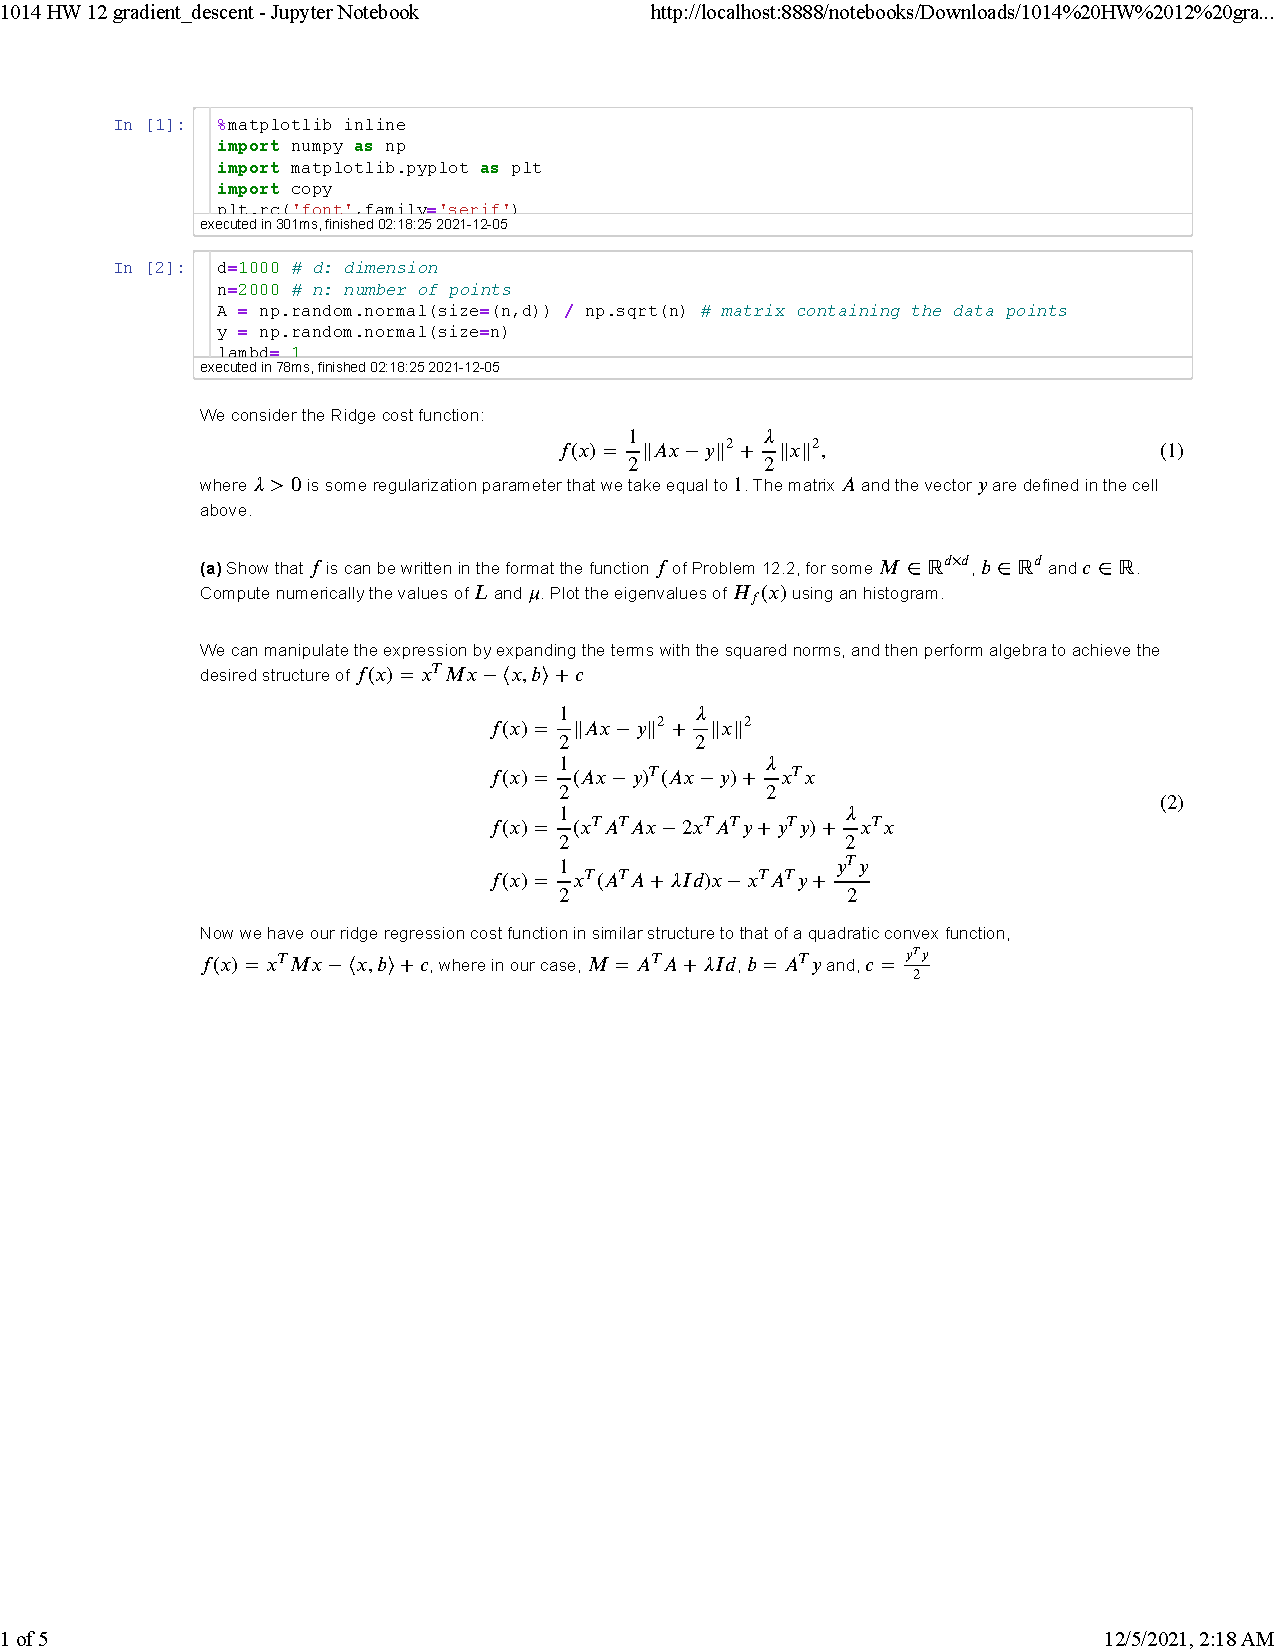
\includepdf[pages=-]{pdf.pdf}


\vspace{5mm}

\section{Problem 12.4}
	We take exactly the same setting of Problem~\ref{p:grad}, but we now consider gradient descent with momentum:
$$
x_{t+1} = x_t - \beta \nabla f(x_t) + \gamma(x_t -x_{t-1}),
$$
for $t \geq 1$,
where we take
$$
\beta = \frac{4}{(\sqrt{L} + \sqrt{\mu})^2}
\qquad \text{and} \qquad
\gamma = \left(\frac{\sqrt{L}-\sqrt{\mu}}{\sqrt{L}+\sqrt{\mu}}\right)^{\! 2}.
$$
Show that the $\alpha_i(t) \defeq \langle v_i, x_t - x^* \rangle$ satisfy a second order linear recurrence relation (as a sequence indexed by $t$). Using this relation, show that for all $t \geq 0$
$$
|\alpha_i(t)| \leq C_i \left(\frac{\sqrt{L}-\sqrt{\mu}}{\sqrt{L} + \sqrt{\mu}}\right)^{\! t}
$$
where $C_i$ is a constant that does not depend on $t$, but that may depend on $x_0,x_1, \mu$ and $L$ (a precise expression of $C_i$ is not expected). Deduce that for all $t \geq 0$
$$
\|x_t - x^*\| \leq C \left(\frac{\sqrt{L}-\sqrt{\mu}}{\sqrt{L} + \sqrt{\mu}}\right)^{\! t}
$$
where $C$ is a constant that does not depend on $t$.


% \newpage
(Help: If you need to get a refresher about what is a linear recurrence, you can check this for instance:
\url{https://www.usna.edu/Users/cs/roche/courses/f19sm242/get.php?f=slides5_8.pdf}. And you should not be afraid of seeing complex numbers showing up.)


%\bibliographystyle{plain}
%\bibliography{./references.bib}
\end{document}
